% Multi-panel figure generated by plot_experiment2_metrics_modelbased.py.
% Requires \usepackage{graphicx} and \usepackage{subcaption}. Paths are
% relative to the repo root (Figs/...); adjust \graphicspath or the paths
% below to match the Overleaf project.
% Include with: % Multi-panel figure generated by plot_experiment2_metrics_modelbased.py.
% Requires \usepackage{graphicx} and \usepackage{subcaption}. Paths are
% relative to the repo root (Figs/...); adjust \graphicspath or the paths
% below to match the Overleaf project.
% Include with: % Multi-panel figure generated by plot_experiment2_metrics_modelbased.py.
% Requires \usepackage{graphicx} and \usepackage{subcaption}. Paths are
% relative to the repo root (Figs/...); adjust \graphicspath or the paths
% below to match the Overleaf project.
% Include with: % Multi-panel figure generated by plot_experiment2_metrics_modelbased.py.
% Requires \usepackage{graphicx} and \usepackage{subcaption}. Paths are
% relative to the repo root (Figs/...); adjust \graphicspath or the paths
% below to match the Overleaf project.
% Include with: \input{experiment2_moredata_modelbased_subopt_gap_figure}
\begin{figure}[htbp]
\centering
\begin{subfigure}[t]{0.48\linewidth}
  \centering
  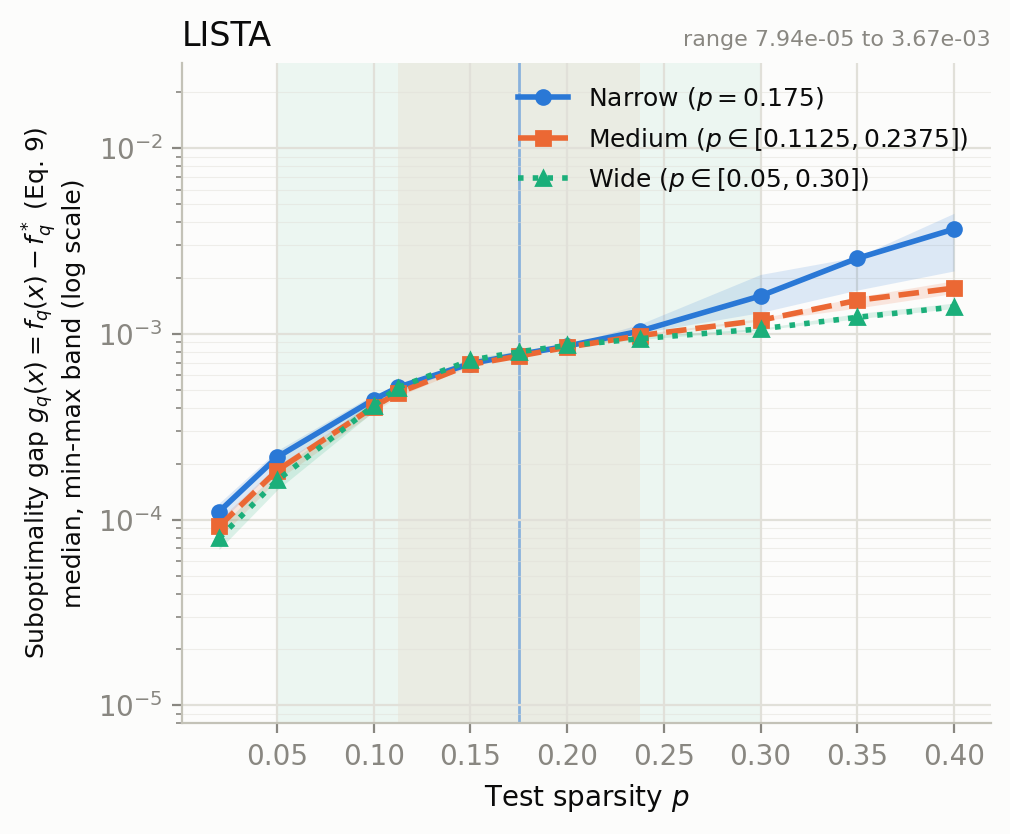
\includegraphics[width=\linewidth]{Figs/experiment2_moredata/experiment2_moredata_modelbased_subopt_gap_lista.png}
  \caption{LISTA}
  \label{fig:experiment2-moredata-modelbased-subopt-gap-lista}
\end{subfigure}\hfill
\begin{subfigure}[t]{0.48\linewidth}
  \centering
  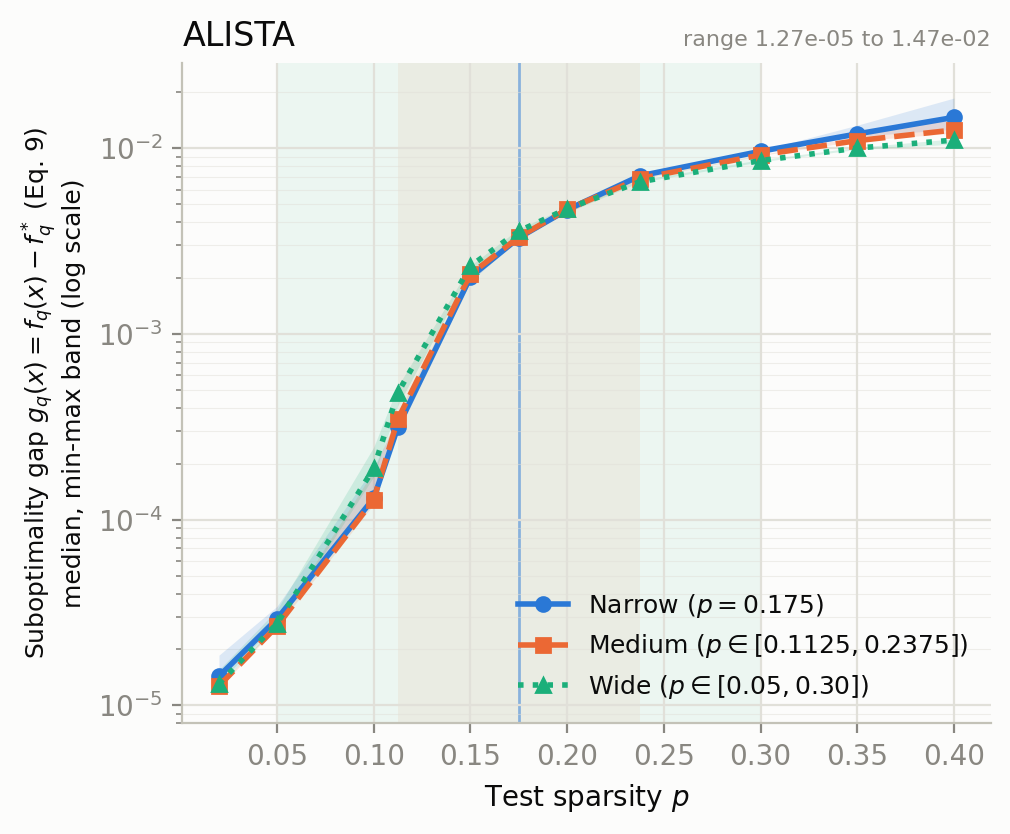
\includegraphics[width=\linewidth]{Figs/experiment2_moredata/experiment2_moredata_modelbased_subopt_gap_alista.png}
  \caption{ALISTA}
  \label{fig:experiment2-moredata-modelbased-subopt-gap-alista}
\end{subfigure}
\caption{Suboptimality gap $g_q(x) = f_q(x) - f^*_q$ (Eq. 9) vs.\ test sparsity $p$, $(m,n) = (25, 50)$, noiseless, 64 000 training instances (2$\times$), 3 seeds. Median over seeds with min-max band; one curve per training-sparsity width, with each width's training support shaded in its colour and the fixed narrow training point marked by a vertical line. Both panels share the y-axis; each panel's own data range is stated in its top-right corner.}
\label{fig:experiment2-moredata-modelbased-subopt-gap}
\end{figure}

\begin{figure}[htbp]
\centering
\begin{subfigure}[t]{0.48\linewidth}
  \centering
  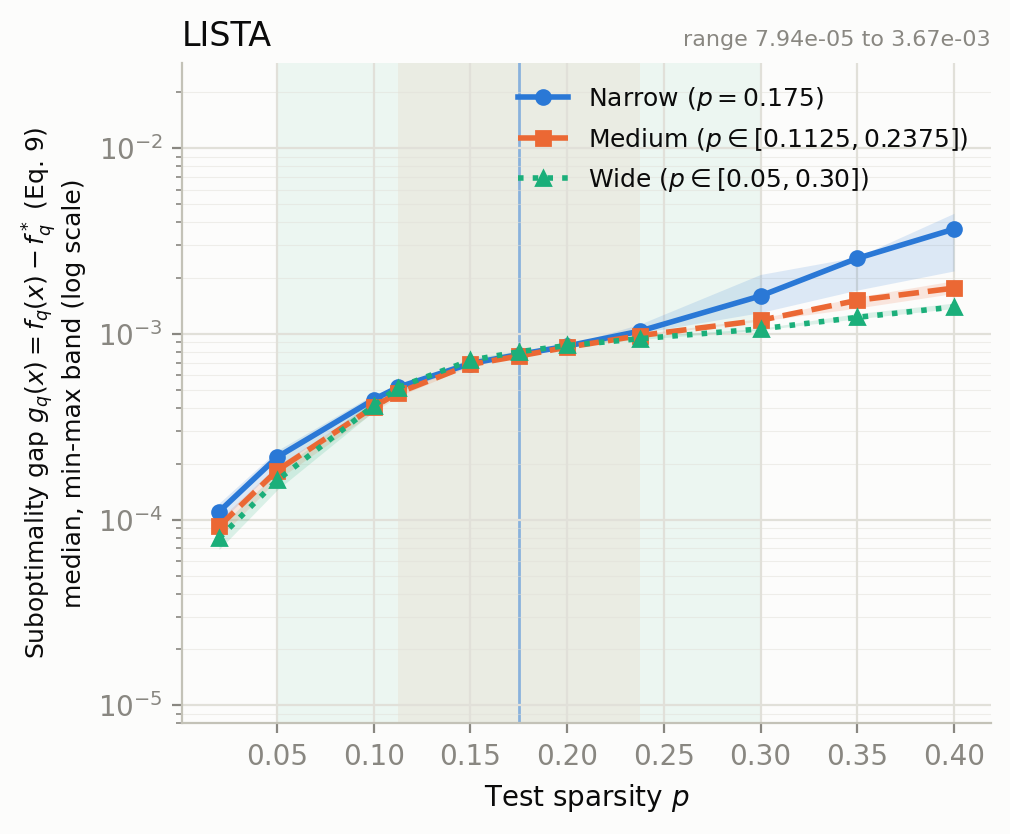
\includegraphics[width=\linewidth]{Figs/experiment2_moredata/experiment2_moredata_modelbased_subopt_gap_lista.png}
  \caption{LISTA}
  \label{fig:experiment2-moredata-modelbased-subopt-gap-lista}
\end{subfigure}\hfill
\begin{subfigure}[t]{0.48\linewidth}
  \centering
  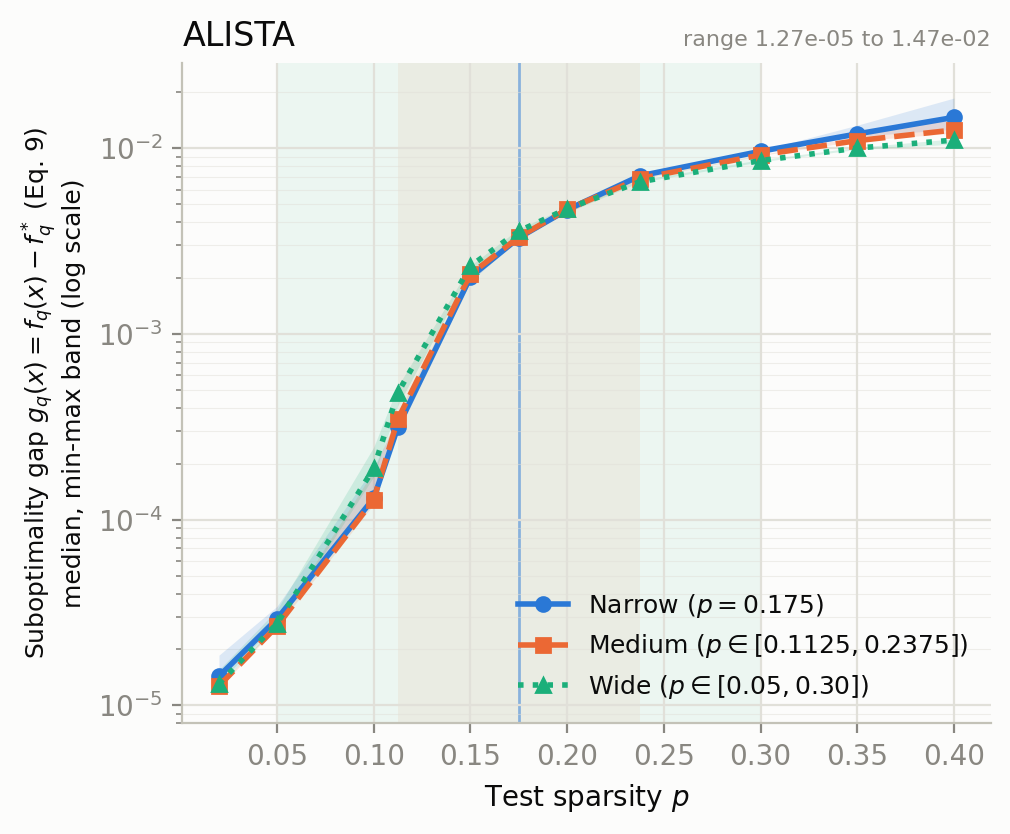
\includegraphics[width=\linewidth]{Figs/experiment2_moredata/experiment2_moredata_modelbased_subopt_gap_alista.png}
  \caption{ALISTA}
  \label{fig:experiment2-moredata-modelbased-subopt-gap-alista}
\end{subfigure}
\caption{Suboptimality gap $g_q(x) = f_q(x) - f^*_q$ (Eq. 9) vs.\ test sparsity $p$, $(m,n) = (25, 50)$, noiseless, 64 000 training instances (2$\times$), 3 seeds. Median over seeds with min-max band; one curve per training-sparsity width, with each width's training support shaded in its colour and the fixed narrow training point marked by a vertical line. Both panels share the y-axis; each panel's own data range is stated in its top-right corner.}
\label{fig:experiment2-moredata-modelbased-subopt-gap}
\end{figure}

\begin{figure}[htbp]
\centering
\begin{subfigure}[t]{0.48\linewidth}
  \centering
  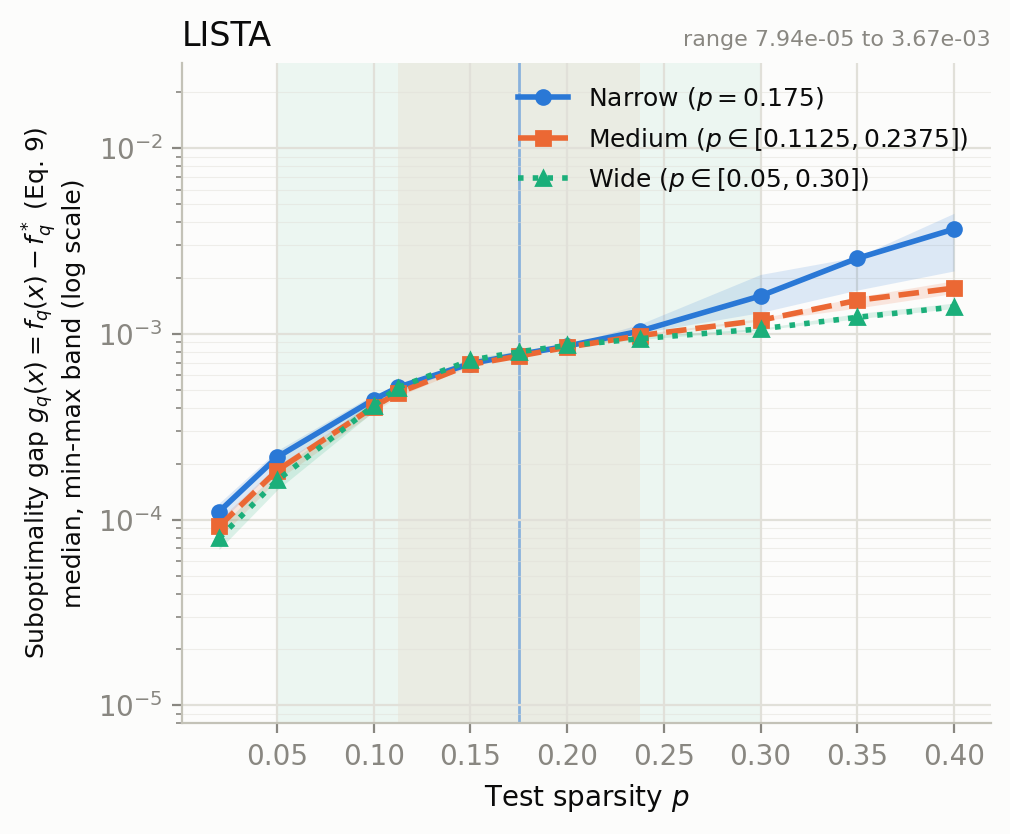
\includegraphics[width=\linewidth]{Figs/experiment2_moredata/experiment2_moredata_modelbased_subopt_gap_lista.png}
  \caption{LISTA}
  \label{fig:experiment2-moredata-modelbased-subopt-gap-lista}
\end{subfigure}\hfill
\begin{subfigure}[t]{0.48\linewidth}
  \centering
  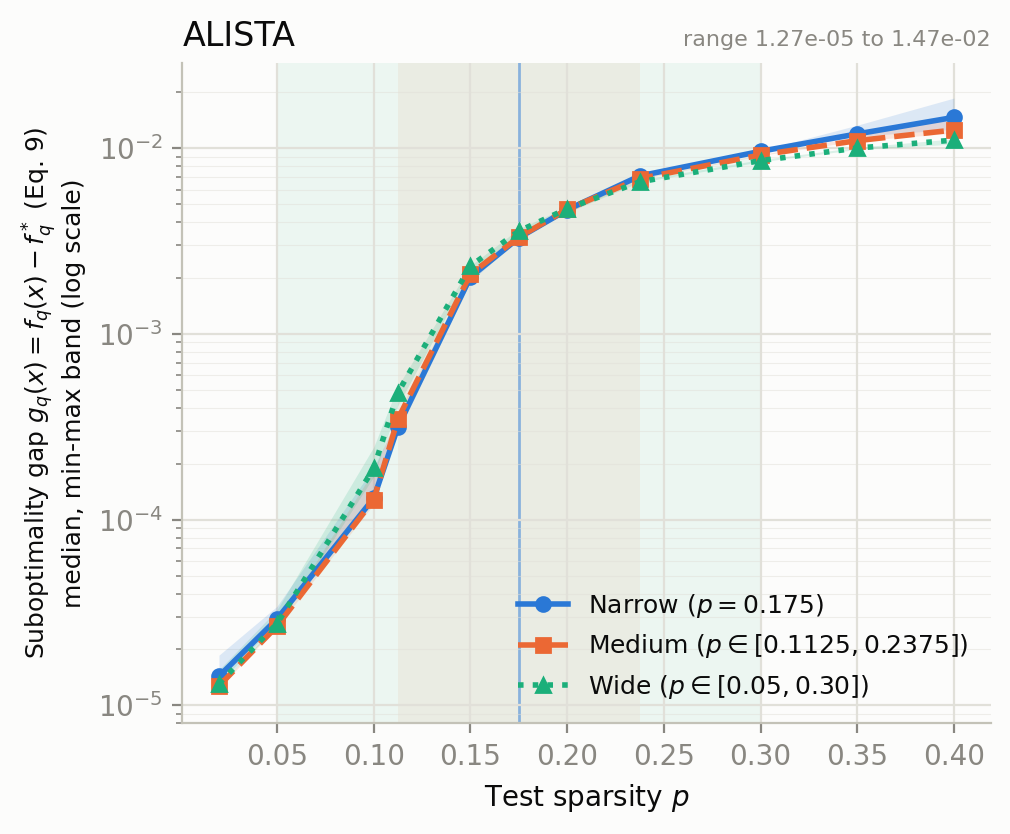
\includegraphics[width=\linewidth]{Figs/experiment2_moredata/experiment2_moredata_modelbased_subopt_gap_alista.png}
  \caption{ALISTA}
  \label{fig:experiment2-moredata-modelbased-subopt-gap-alista}
\end{subfigure}
\caption{Suboptimality gap $g_q(x) = f_q(x) - f^*_q$ (Eq. 9) vs.\ test sparsity $p$, $(m,n) = (25, 50)$, noiseless, 64 000 training instances (2$\times$), 3 seeds. Median over seeds with min-max band; one curve per training-sparsity width, with each width's training support shaded in its colour and the fixed narrow training point marked by a vertical line. Both panels share the y-axis; each panel's own data range is stated in its top-right corner.}
\label{fig:experiment2-moredata-modelbased-subopt-gap}
\end{figure}

\begin{figure}[htbp]
\centering
\begin{subfigure}[t]{0.48\linewidth}
  \centering
  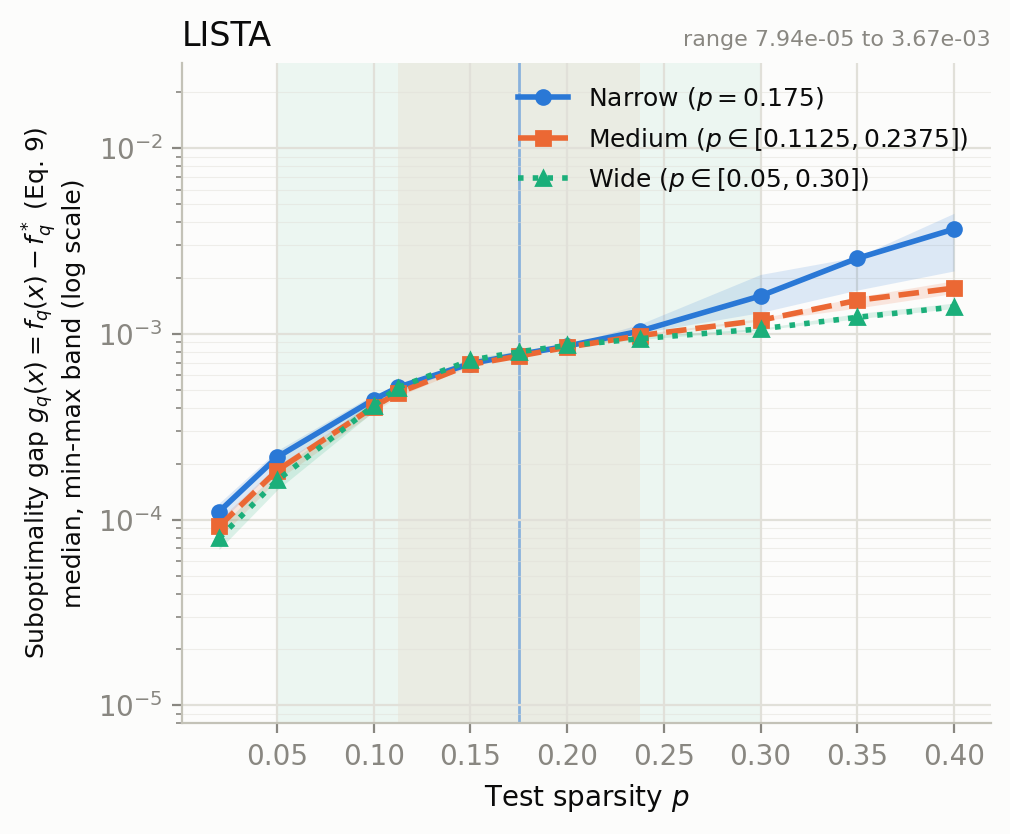
\includegraphics[width=\linewidth]{Figs/experiment2_moredata/experiment2_moredata_modelbased_subopt_gap_lista.png}
  \caption{LISTA}
  \label{fig:experiment2-moredata-modelbased-subopt-gap-lista}
\end{subfigure}\hfill
\begin{subfigure}[t]{0.48\linewidth}
  \centering
  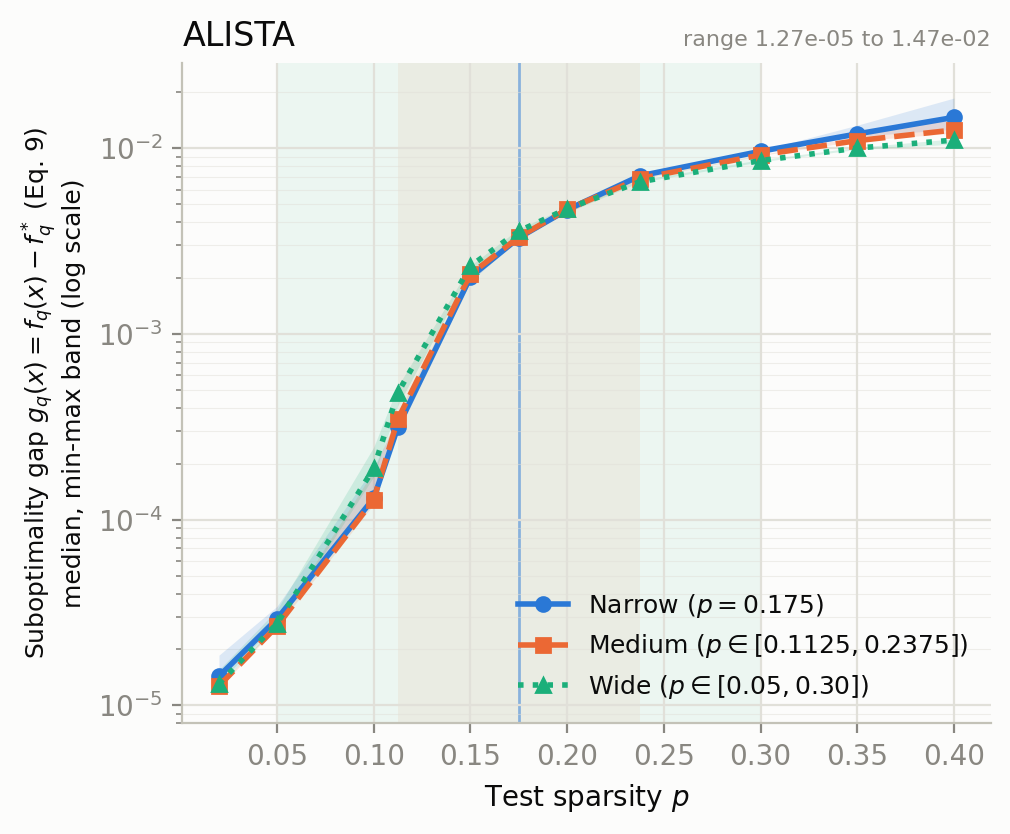
\includegraphics[width=\linewidth]{Figs/experiment2_moredata/experiment2_moredata_modelbased_subopt_gap_alista.png}
  \caption{ALISTA}
  \label{fig:experiment2-moredata-modelbased-subopt-gap-alista}
\end{subfigure}
\caption{Suboptimality gap $g_q(x) = f_q(x) - f^*_q$ (Eq. 9) vs.\ test sparsity $p$, $(m,n) = (25, 50)$, noiseless, 64 000 training instances (2$\times$), 3 seeds. Median over seeds with min-max band; one curve per training-sparsity width, with each width's training support shaded in its colour and the fixed narrow training point marked by a vertical line. Both panels share the y-axis; each panel's own data range is stated in its top-right corner.}
\label{fig:experiment2-moredata-modelbased-subopt-gap}
\end{figure}
